% \documentclass[10pt,a4paper]{article}
% \include{header}
% \appendtographicspath{{/home/debortoli/research/patch_sim/res/res_internal_percep/}{/home/debortoli/research/patch_sim/res_percep/}{/home/debortoli/research/patch_sim/res/}{./eps2pdf/}}
% \bibliography{/home/debortoli/research/research.bib}
% \title{Patch similarity} \author{Valentin De Bortoli}
% \begin{document}
\section{Patch similarity functions}
%{{{ introduction

The different possibilities for $\Omega$ will be studied in this document. $u^0$ will be a
template image also defined on $\Omega$.  Both $u^0$ and $u$ take their values
in $\mathbb{R}$.  In this section we investigate patch similarity functions.  Our
goal is to find a similarity function which is tractable with an \acontrario \
setting and presents good visual properties. To our knowledge there exists no
review on the subject. We are looking for similarity functions which do not use
a probabilistic background since this background will be introduced using an
\acontrario \ model. In \cite{deledalle2012compare} the authors present similarity functions but most
of them are based on a frequentist or bayesian approach thus not appropriate in
our setting. Some popular patch similarity functions are based on modified euclidean distances, $i.e$ positive definite quadratic forms. This approach was used in denoising applications \cite{buades2005non}. In \cite{delon2013patch}, the authors derived optimal weights to discriminate identical patches. \\
\comment{ (10/10) j'ai posé la question à Sivic qui, en cours d'object
  recognition, parle de norme euclidienne entre des patches. A sa connaissance à
  part la cross-correlation il n'y a pas d'autres normes typiques utilisées (du
  moins qui lui venait directement à l'esprit lorsque je lui ai posé la
  question). Néanmoins il m'a dit (et j'ai pu constater en faisant une petite
  recherche bibliographique) que de nouvelles fonctions de similarité étaient
  déterminées \textit{via} du learning. Peut-être que ces fonctions pourraient
  être calculées dans un premier temps puis utilisées dans le cadre \acontrario
  . Faut-il évoquer d'autres mesures plus empiriques comme SSIM ?}
\\
\comment{ (30/10) parler des espaces à noyaux et des calculs dans ces espaces.
  On peut aussi parler de l'utilisation de normes différentes de la norme 2 pour
  obtenir des contraines de sparsité}
These patch similarity functions will be used in two different settings:
\begin{itemize}
\item \textit{internal matching:}
  $s\left(u(\mathcal{P}), \tau_t(u)(\mathcal{P})\right)$ measures the similarity
  between a patch in $u$ and its shifted version in $u$.  In an \acontrario \
  setting an offset $t$ will be detected if a patch and its shifted version
  present a similarity which is not likely to be present in the background
  stochastic model.  This can be used in periodicity analysis or in a
  variational context.
\item \textit{template matching:}
  $s\left(u^0(\mathcal{P}), \tau_t(u)(\mathcal{P}) \right)$ measures the
  similarity between a patch template and the patches in $u$. In an \acontrario \
  setting \ $u$ can be generated as a textured version of
  $u^0(\mathcal{P})$. This similarity function can be used in a discriminative,
  or parametric, texture synthesis algorithm.  The terminology \textit{template
    matching} was introduced in \cite{deledalle2012compare}.
\end{itemize}
Now we want to investigate patch similarity functions which are tractable in the
sense that either $s\left(u(\mathcal{P}), \tau_t(u)(\mathcal{P})\right)$ or
$s\left(u^0(\mathcal{P}), \tau_t(u)(\mathcal{P})\right)$ probability density
functions can be computed. We need to precise the underlying stochastic process
$u$. Usually $u$ will be a white noise, a \DSN \ model or an \ADSN \ model.\\
\comment{(10/10) d'autres modèles à voir ? \\
(30/10) d'autres références pour la comparaison entre patchs ?} Tractability issues occur only
considering discretizations of our setting. Thus we will not bother considering
these issues in the continuous domain.  However it will still be of interest to
derive properties in the continuous domain. Table \ref{tab:patch_sim} gives a brief summary of
the similarity functions studied in this report and their properties.
% EN LIGNES LES DIFFERENTES DISTANCES QUI PEUVENT ETRES UTILISÉES PDF ?
% PROPERTIES
\begin{table}[h]
  \begin{tabularx}{\textwidth}{|c||X|X|}
    \hline
    \diagbox{similarity \newline functions}{matching case}         & Internal matching               & Template matching               \\ \hline \hline
    $s_{\|\cdot\|,2}(A,B) = \| A-B \|_2$                           & non-asymptotic expression       & non-asymptotic expression       \\ \hline
    $s_{\langle \cdot\rangle,2}(A,B) = \langle A,B \rangle$        & asymptotic expression, Gaussian & asymptotic expression, Gaussian \\ \hline
    $s_{\cos,2}(A,B) = \frac{\langle A,B \rangle}{\|A\|_2\|B\|_2}$ & asymptotic expression, Gaussian & asymptotic expression, Gaussian \\ \hline
    $s_{\|\cdot\|, 1}(A,B) = \| A-B \|_1$                          & not tractable                   & not tractable                   \\ \hline
    $s_{\|\cdot\|,\infty}(A,B) = \| A-B \|_{\infty}$               & not tractable                   & not tractable                   \\ \hline    
  \end{tabularx}
  \caption{A summary of the properties of the different patch similarity functions investigated}
  \label{tab:patch_sim}
\end{table}
\subparagraph{Features} We compute the patch similarity functions quantity
directly on patch pixel values. It can be interesting to compute features on the
images and then make use of the patch similarity function.  For example in \cite{patraucean2013detection} the authors compute the gradient of the original image. The model image is a
white noise and thus looking at the orientation of its gradient we obtain an
uniform probability density function. To be precise if the gradient is computed
using finite differences the gradient is computed in the model image on a
thinner grid (or is computed exactly in a continuous setting), otherwise the
gradient orientations are not independent. Linear filtering is another
option. One could note that in a centered Gaussian case this simply amounts to
changing the covariance function.  \subparagraph{} In the following subsection
we give details about the results stated in Table \ref{tab:patch_sim}. For every similarity
function we try to give results for the different probabilistic settings and
$\Omega$ set.

%}}}
%{{{ a contrario setting
\subsection{ \acontrario \ setting}
We restrict ourselves to $\Omega_{m,n} := \mathbb{T}_m \times \mathbb{T}_n$, the set of definition of discrete periodic images. For
implementation purposes this framework will be chosen. However the periodic
assumption is not always satisfied. Several solutions exist to project periodic
functions onto the set of the periodic functions \cite{moisan2011periodic}, however they all suffer
from drawbacks. This problem will not be addressed here.
%{{{ s2 patch similarity function
\subsubsection{\s2
  patch similarity function} We will not study \s2 directly but
$s_2 = s_{\| \cdot \|, 2} ^2$. Before stating a few results let us introduce some
notions.
\begin{mydef}[Autocorrelation]
  Let $h$ defined on $\Omega$. We define the autocorrelation $A_h$ on $\Omega$,
  \[A_h = h * \check{h} \] Note that $A_h$ takes real values and is
  symmetric.
\end{mydef}
Note that since $h$ was defined on a finite grid no assumption was needed on $h$. Suppose $h$ was defined on $\mathbb{Z}^2$ then the natural hypothesis is $h \in \ell^2(\Omega)$.
Let us focus on the \internalmatching . We derive the following property.
\begin{prop}
  Let $u$ be a Gaussian field on $\Omega$ with mean $0$ and covariance matrix
  $C$, then
  \[s_2\left(u(\mathcal{P}), \tau_t(u)(\mathcal{P})\right) \sim \summ{x \in
      \mathcal{P}}{}{\lambda_x \xi_x}\] where $(\xi_x)_{x \in \mathcal{P}}$ are
  independent chi-square variables with one degree of freedom and
  $(\lambda_x)_{x \in \mathcal{P}}$ are the eigenvalues of
  $\Gamma_{\mathcal{P}} \in \mathcal{M}_{\vert \mathcal{P} \vert}\left(
    \mathbb{R} \right)$, with
  \[ \Gamma_{\mathcal{P}}(x,x') = C(x, x') + C(t+x, t+x') - C(x,t+x') -
    C(x+t,x').
  \]
  \label{p:s2internal}
\end{prop}
We must distinguish two cases:
\begin{itemize}
\item white noise case $C(x,x') = \delta_{x,x'}$ and
  $\Gamma_{\mathcal{P}} = 2\delta_{x,x'} - \delta_{x,x'+t} - \delta_{x,x'-t}$,
\item \ADSN \ case where $C(x,x') = A_h(x-x')$ ($h$ is a function defined on
  $\Omega$) and
  \[\Gamma_{\mathcal{P}} = 2A_h(x-x') - A_h(x-x'-t) - A_h(x-x'+t) .\]
\end{itemize}
In both cases $\Gamma_{\mathcal{P}}$ is block symmetric with symmetric blocks, positive semi-definite and Toeplitz with Toeplitz blocks. Eigenvalues can be computed using a block circulant with circulant blocks approximation and in the white noise case closed forms can be derived for the eigenvalues. Another problem is sampling a weighted sum of independent chi-square variables. A large literature exists on the subject \cite{wood1989f}, \cite{moschopoulos1984distribution}, \cite{box1954some}, \cite{imhof1961computing}, \cite{jensen1972gaussian}, \cite{kotz1967series}, \cite{bodenham2016comparison}.\\
Now we present results in \templatematching .
\begin{prop}
  Let $u$ be a Gaussian field on $\Omega$ with mean $0$ and covariance matrix
  $C$, then
  \[s_2\left(u^0(\mathcal{P}), \tau_t(u)(\mathcal{P}) \right) \sim \summ{x \in
      \Omega}{}{\lambda_x}{\tilde{\xi}_x}\] where
  $\left( \tilde{\xi}_x\right)_{x\in \mathcal{P}}$ are independent non centered
  chi-square variables with one degree of freedom and non centering parameter
  $\left(-P_t u^0(\mathcal{P}) (x) \right)_{x \in \mathcal{P}}$ where
  $P_t \in \mathcal{O}_{\vert \mathcal{P} \vert}\left( \mathbb{R} \right)$ such
  that $P_t D P_t^T = C_{\tau_{-t}\left(\mathcal{P}\right)}$
  ($C_{\tau_{-t}\left(\mathcal{P}\right)}$ is the restriction of $C$ to the
  $\tau_{-t}\left(\mathcal{P}\right)$ indices) and where
  $(\lambda_x)_{x\in\tau_{-t}\left(\mathcal{P}\right)}$ are the eigenvalues of
  $C_{\tau_{-t}\left(\mathcal{P}\right)}$.
  \label{s2template}
\end{prop}
In the special case where $u$ is a white noise, $P_t$ is the identity matrix and ${\forall x \in \mathcal{P}, \lambda_x = 1}$. As before there exists techniques to easily compute approximations of the eigenvalues of the restricted matrices. The main difficulty is to sample from a weighted sum of non centered independent chi-square random variables.\\
\comment{(10/10) je devrais procéder à une bibliographie sur le sujet mais des
  techniques issues du cas centré peuvent être exportées dans le cas non
  centrés, je pense à Imhof notamment.}
%}}}
%{{{ sps patch similarity function

\subsubsection{\sps \ patch similarity function} Since template matching is intractable
in the \s2 \ case we only consider the scalar product. The idea of considering scalar product
instead of Euclidean norm can be found in \cite{riot2017correlation}. Concerning the
\internalmatching \ \sps \ seems intractable. Indeed denoting
$p_{\mathcal{P}} \in \mathcal{M}_{\vert \mathcal{P} \vert, \vert \Omega
  \vert}\left( \mathbb{R} \right)$ the projection matrix onto the subspace
spanned by $(u(x))_{x\in \mathcal{P}}$ we obtain that
\[s_{\langle \cdot \rangle, 2}\left(u(\mathcal{P}),
    \tau_t(u)(\mathcal{P})\right) = u^T p_{\mathcal{P}}^T
  p_{\tau_t(\mathcal{P})} u\] Let
$A = p_{\mathcal{P}}^T p_{\tau_t(\mathcal{P})}$. $A$ is not symmetric and we
even have
\[ \ AA^T = \summ{x \in \mathcal{P}}{}E_{x,x}, \ \text{and} \ A^TA = \summ{x \in \mathcal{P}}{}E_{x+t,x+t},\]
where $(E_{x,y})_{(x,y) \in \Omega^2}$ is the canonical basis of $\mathcal{M}_{\vertt{\Omega}}\left(\mathbb{R}\right)$.
Thus $A$ is not normal and cannot be diagonalized using orthonormal
matrices. Thus \sps \ cannot be written as a weighted sum of chi-square random
variables. This conclusion holds for every Gaussian field with mean $0$. However
asymptotic results can be derived.
\begin{prop}
  Let $u$ be a Gaussian field defined on $\mathbb{Z}^2$. We define
  $\left(u_k\right)_{k \in \mathbb{N}}$ the sequence of Gaussian fields
  defined by the restriction of $u$ to $\llbracket 1,M_k \rrbracket \times \llbracket 1,N_k \rrbracket$. We suppose $u$ is
  stationary and its covariance matrix is given by
  $\forall (x,x') \in \mathbb{Z}^2, \ C(x,x') = R_u(\vertt{x-x'}) =
  A_h(x-x')$. We also suppose that $h$ has compact support. Let
  $\seq{\mathcal{P}}{k}$ be a sequence of increasing sets such that
  $\mathcal{P}_k \subset \llbracket 1,M_k \rrbracket \times \llbracket 1,N_k \rrbracket$ then we have
  \[\vertt{\mathcal{P}_k}^{-1} s_{\langle \cdot
      \rangle,2}\left(u_k(\mathcal{P}_k),
      \tau_t(u_k)(\mathcal{P}_k) \right) \ \underset{k
      \rightarrow +\infty}{\overset{\text{a.s}}{\longrightarrow}} A_h(t).\]\label{p:sps_internal_as}
\end{prop}
In order to sample we can use Proposition \ref{p:ADSN_restriction_Z2}.
\begin{proof}
  $s_{\langle \cdot \rangle,2}\left(u_k(\mathcal{P}_k),
    \tau_t(u_k)(\mathcal{P}_k) \right) = \summ{x \in
    \mathcal{P}_k}{}{u(x)u(x+t)}$. Let us denote $Y(x) = u(x)u(x+t)$. We have
  $\forall x \in \mathbb{Z}^2, \ E(Y(x)) = A_h(t)$. We also have
  \[E(Y(x)Y(x')) = E(u(x)u(x+t)u(x')u(x'+t)) = A_h(t)^2 + A_h(x-x')^2 +
    A_h(x-x'+t)A_h(x-x'-t),\] using Isserlis theorem. Thus
  $\text{Cov}(Y(x)Y(x')) = A_h(x-x')^2 + A_h(x-x'+t)A_h(x-x'-t)$. For $x-x'$
  large enough the covariance is zero since $h$ has compact support.  Thus the
  strong law of large numbers for weakly correlated $L^2$ random variables apply
  and we can conclude, see \cite{bernstein1927extension}.
\end{proof}

\begin{prop}
  Let $(u_k)_{k \in \mathbb{N}}$ and
  $\left(\mathcal{P}_k\right)_{k \in \mathbb{N}}$ defined as in Proposition \ref{p:sps_internal_as}. We have
  \[\frac{1}{ \sqrt{\vertt{\mathcal{P}_k}\sigma^2}} \left(s_{\langle \cdot
        \rangle,2}\left(u_k(\mathcal{P}_k),
        \tau_t(u_k)(\mathcal{P}_k) \right) -
      \vertt{\mathcal{P}_k}A_h(t)\right) \ \underset{k \rightarrow
      +\infty}{\overset{\mathcal{L}}{\longrightarrow}} \ \mathcal{N}(0,1),\]
  where
  $\sigma^2 = 2 \left( \| A_h \|_2^2 + \summ{x \in
      \mathbb{Z}^2}{}{A_h(x+t)A_h(x-t)}\right) - A_h(0)^2 - A_h(t)^2.$
  \label{p:spsinternal}
\end{prop}
\begin{proof}
  This is a simple application of the Central Limit Theorem with mixing
  conditions see \cite{billingsley2013convergence} for more details. Note that
  here we are in the $m-$dependency case, i.e for large enough offsets the mixing
  number is zero. Since $Y(x)$ admits moments at every order we can apply the
  theorem.
\end{proof}
\remark{
  It is interesting to note that the mixing conditions introduced in this proof are also used in \cite{levina2006texture} to show that the Efros-Leung algorithm introduced in \cite{efros1999texture} converges.}\\
The case of \templatematching \ is far more simpler.
\begin{prop}
  Let $u$ be a Gaussian field on $\Omega$ with mean $0$ and covariance $C$ then,
  \[s_{\langle \cdot \rangle, 2}\left( u^0(\mathcal{P}),
      \tau_t(u)(\mathcal{P})\right) \sim \mathcal{N}\left(0,\summ{x,x' \in
        \mathcal{P}^2}{}{u^0(x)u^0(x')C(x+t,x'+t)} \right).\]
  \label{p:spstemplate}
\end{prop}
Suppose also $u$ is stationary then there exists $R_u$ such that
$C(x,x') = R_u(x-x')$. In this case,
\[\summ{x,x' \in \mathcal{P}^2}{}{u^0(x)u^0(x')C(x+t,x'+t)} = \langle
  \mathbb{1}_{\cdot \in \mathcal{P}}u^0, \left(\mathbb{1}_{\cdot \in
      \mathcal{P}}u^0\right) * R_u\rangle.\] To derive results in the \scos \
patch similarity function case we also need asymptotic results. Using the strong
law of large numbers for weakly correlated $L^2$ random variables and Central
Limit Theorem with mixing conditions we obtain the following results.
\begin{prop}
  Let $\seq{u}{k}$ and $\seq{\mathcal{P}}{k}$ defined as in Proposition \ref{p:sps_internal_as}.
  We have
  \[
    \vertt{\mathcal{P}_k}^{-1} s_{\langle \cdot \rangle,2} \left(u_k^0(\mathcal{P}_k), \tau_t(u_k)(\mathcal{P}_k) \right) \
    \overset{\text{a.s}}{\underset{k \rightarrow +\infty}{\longrightarrow}} 0,\]
  and
  \[
    \frac{1}{\sqrt{\vertt{\mathcal{P}_k} \sigma^2}} s_{\langle \cdot \rangle,2}
    \left(u_k^0(\mathcal{P}_k), \tau_t(u_k)(\mathcal{P}_k) \right) \
    \overset{\mathcal{L}}{\underset{k \rightarrow +\infty}{\longrightarrow}}
    \mathcal{N}(0,1),\] where
    $\sigma^2 = 2 \left(\|A_h\|_2^2 + \summ{x \in
      \Omega}{}{A_h(x+t)A_h(x-t)}\right) - A_h(t)^2 - A_h(0)^2$.
\label{p:spstemplateasymp}
\end{prop}
\remark{Note that Proposition \ref{p:spstemplate} applies on every $\Omega$, finite or not. This is not
the case in the asymptotic case where $\Omega = \mathbb{Z}^2$. In the general case, all asymptotic results are derived with $h$ defined over $\mathbb{Z}^2$.}

%}}}
%{{{ scos patch similarity function

\subsubsection{\scos \ patch
  similarity function} We try to derive \internalmatching \ and
\templatematching \ p.d.f using the \scos \ patch similarity function. There is
little hope to obtain closed forms in the general case but asymptotic results
can be derived easily.

\begin{prop}
    Let $u$ be a Gaussian field defined on $\mathbb{Z}^2$. We define
  $\left(u_k\right)_{k \in \mathbb{N}}$ the sequence of Gaussian fields
  defined by the restriction of $u$ to $\llbracket 1,M_k \rrbracket \times \llbracket 1,N_k \rrbracket$. We suppose $u$ is
  stationary and its covariance matrix is given by
  $\forall (x,x') \in \mathbb{Z}^2, \ C(x,x') = R_u(\vertt{x-x'}) =
  A_h(x-x')$. We also suppose that $h$ has compact support. Let
  $\seq{\mathcal{P}}{k}$ be a sequence of increasing sets such that
  $\mathcal{P}_k \subset \llbracket 1,M_k \rrbracket \times \llbracket 1,N_k \rrbracket$ then we have that
  $s_{\cos,2}(u_k(\mathcal{P}_k),
  \tau_t\left(u_k\right)(\mathcal{P}_k))$ is defined almost everywhere and,
  \[
    \sqrt{\frac{\vert \mathcal{P}_k \vert}{\sigma^2}} \
    \left(s_{\cos,2}(u_k(\mathcal{P}_k), \tau_t
    \left(u_k\right)(\mathcal{P}_k)) - \frac{A_h(t)}{A_h(0)} \right) \ \overset{\mathcal{L}}{\underset{k
        \rightarrow +\infty}{\longrightarrow}} \ \mathcal{N}(0,1).
  \]
  where
  $\sigma^2 = \frac{1}{A_h(0)^2}\left(2 \left(\|A_h\|_2^2 + \summ{x \in
      \Omega}{}{A_h(x+t)A_h(x-t)}\right) - A_h(t)^2 - A_h(0)^2\right)$.
  \label{p:scosinternal}
\end{prop}
\begin{prop}[Almost sure convergence]
  Under the same hypotheses of Proposition \ref{p:scosinternal} we have
  \[ s_{\cos, 2} \left( u_{
        M_k,N_k}(\mathcal{P}_k),\tau_t(u_k)(\mathcal{P}_k)\right) \
    \overset{\text{a.s}}{\underset{k \rightarrow +\infty}{\longrightarrow}} \
    \frac{A_h(t)}{A_h(0)} \]
  The convergence also occurs in $L^1$ since the sequence is bounded by $1$.
\end{prop}

\begin{prop}
  Let $\seq{u}{k}$ and $\seq{\mathcal{P}}{k}$ defined as in Proposition \ref{p:scosinternal}.
We  also suppose that $h$ has compact support, $u_{k}^0$ a sequence of
  images defined over $\llbracket 1,M_k \rrbracket \times \llbracket 1,N_k \rrbracket$ such that $\| u_k^0 \|_2 =
  1$. Let $\seq{\mathcal{P}}{k}$ be a sequence of increasing sets such that
  $\mathcal{P}_k \in \Omega_{M_k,N_k}$ then
  $s_{\cos,2}(u_k^0(\mathcal{P}_k), u_k(\mathcal{P}_k))$ is
  defined almost everywhere and we have
  \[
    \sqrt{\frac{\vert \mathcal{P}_k \vert}{\sigma^2}} \ s_{\cos,2}(u_k^0(\mathcal{P}_k), u_k(\mathcal{P}_k)) \
    \overset{\mathcal{L}}{\underset{k \rightarrow +\infty}{\longrightarrow}} \
    \mathcal{N}(0,1).
  \]
  where
  $\sigma^2 = \langle \mathbb{1}_{\cdot \in \mathcal{P}}u^0,
  \left(\mathbb{1}_{\cdot \in \mathcal{P}}u^0\right) * \frac{A_h}{A_h(0)}\rangle$.
  \label{p:scostemplate}
\end{prop}
\begin{proof}
  $s_{\langle \cdot \rangle, 2}\left( u^0(\mathcal{P}),
    \tau_t(u)(\mathcal{P})\right) \sim \mathcal{N}\left(0,\summ{x,x' \in
      \mathcal{P}^2}{}{u^0(x)u^0(x')A_h(x-x')} \right)$ and
  \[\vertt{\mathcal{P}_k}^{-1}
    s_{2}(u_k(\mathcal{P}_k),u_k(\mathcal{P}_k)) =
    \vertt{\mathcal{P}_k}^{-1} s_{\langle \cdot
      \rangle,2}\left(u_k(\mathcal{P}_k),
      \tau_t(u_k)(\mathcal{P}_k) \right) \ \underset{k
      \rightarrow +\infty}{\overset{\text{a.s}}{\longrightarrow}} A_h(0)\] We
  conclude using Slutsky theorem.
  % There exists an isometric transform, $f_k$ over $\Omega_{M_k,N_k}$, such
  % that
  % $f_k(u_{0 M_k,N_k}(\mathcal{P}_k)) = \delta_{x_k}$ with
  % ${x_k \in \mathcal{P}_k}$. Therefore, since $f_k$ is isometric,
  % \[s_{\langle \cdot \rangle,2}\left(u_{0 M_k,N_k}(\mathcal{P}_k),
  %     u_k(\mathcal{P}_k) \right) = s_{\langle \cdot
  %   \rangle,2}\left(f_k\left(u_{0 M_k,N_k}(\mathcal{P}_k)\right),
  %     f_k\left(u_k(\mathcal{P}_k)\right) \right).\] Note that
  % $f_k\left(u_k(\mathcal{P}_k)\right)$ is still a white noise. Thus
  % \[s_{\langle \cdot \rangle,2}\left(f_k\left(u_{0
  %       M_k,N_k}(\mathcal{P}_k)\right),
  %     f_k\left(u_k(\mathcal{P}_k)\right) \right) \sim
  %   \mathcal{N}(0,1).\] Moreover
  % $\frac{\summ{x \in \mathcal{P}_k}{}{u_k(x)^2}}{\vert \mathcal{P}_k
  % \vert}$ is the empirical mean of independent integrable variables and the
  % strong law of large numbers give
  % ${\frac{\summ{x \in \mathcal{P}_k}{}{u_k(x)^2}}{\vert \mathcal{P}_k
  % \vert} \ \underset{k \rightarrow +\infty}{\longrightarrow} \
  % E(u_{M_0,N_0}(0)^2) = 1}$. We use the Slutsky theorem to conclude.
\end{proof}
\begin{prop}[Almost sure convergence]
  Under the same hypotheses of Proposition \ref{p:scostemplate}, we have
  \[ s_{\cos, 2} \left( u_k^0(\mathcal{P}_k),u_k(\mathcal{P}_k)\right) \
    \overset{\text{a.s}}{\underset{k \rightarrow +\infty}{\longrightarrow}} \
    0. \]
  Once again the convergence also occurs in $L^1$ since the sequence is bounded.
\end{prop}
% \begin{proof}
%   We note
%   $s_k = s_{\cos, 2} \left( u_{0,
%       M_k,N_k}(\mathcal{P}_k),u_k(\mathcal{P}_k)\right)$. Let
%   $a \in \mathbb{R}_+^*$, we have
%   \[
%     P\left(\vertt{s_k} \ge a\right) \le \frac{E(s_k^2)}{a^2},
%   \]
%   thanks to the Markov inequality. We now estimate the expectation
%   \[
%     \al{
%       E(s_k^2) &= \frac{1}{(2\pi)^{\frac{p_k}{2}}} \intt{(x_i)_{i \in \llbracket 1,p_k \rrbracket} \in \mathbb{R}^{p_k}}{}{\frac{x_1^2}{x_1^2 + \dots + x_{p_k}^2}\exp(-\frac{x_1^2 + \dots x_{p_k}^2}{2})}{x_1}\dots\text{d}x_{p_k} \\
%       &=  \frac{1}{(2\pi)^{\frac{p_k}{2}}}\intt{R \in \mathbb{R_+^*}, (\theta_1, \dots, \theta_{p_k-2}) \in [0,\pi]^{n-2}, \theta_{p_k-1} \in [-\pi,\pi]}{}{\frac{R^2 \cos(\theta_1)^2 \dots \cos(\theta_{p_k-1})^2}{R^2} \exp(-\frac{R^2}{2})R}{R} \text{d}\theta_1 \dots \text{d}\theta_{n-1} \\
%       &\le \frac{\tilde{C}}{(2\pi)^{\frac{p_k}{2}}} \left( \intt{0}{\pi}{\cos(\theta)^2}{\theta}\right)^{p_k -1} \\
%       &\le C \left( \frac{\sqrt{\pi}}{2 \sqrt{2}} \right)^{p_k -1}, }
%   \]
%   where $C$ and $\tilde{C}$ are positive constants.
%   $\kappa = \frac{\sqrt{\pi}}{2 \sqrt{2}} <1$. Thus,
%   $P\left(\vertt{s_k} \ge a\right) \le C \kappa^k$ and
%   $\left(P\left( \vertt{s_k} \ge a \right)\right)_{k \in \mathbb{N}}$ is
%   summable for each $a \in \mathbb{R}_+^*$. We can conclude that $s_k$ converges
%   to zero almost surely.
% \end{proof}
 \remark{
  We suppose we have one realization of a white noise and then we make $(M,N)$ go to infinity. It is not sure what happens if we decide to use a new independent white noise defined over $\llbracket 1,M_k \rrbracket \times \llbracket 1,N_k \rrbracket$ for each couple $(M_k,N_k)$. As noted by Terrence Tao in  \url{https://terrytao.wordpress.com/2008/06/18/the-strong-law-of-large-numbers/} recycling the random variables is crucial in the approximation process. However the theorem is valid if the sequence $\left(\vertt{\mathcal{P}_n}\right)_{n \in \mathbb{N}}$ in the sense that there exists some constant $c>1$ such that $ \frac{\vertt{\mathcal{P}_{n+1}}}{\vertt{\mathcal{P}_n}} > c$. In the case of a lacunary sequence we do not need to first define a discrete field over $\mathbb{Z}^2$ but can proceed with Gaussian vectors onto $\llbracket 1,M_k \rrbracket \times \llbracket 1,N_k \rrbracket $.}\\

%}}}
%{{{ other similarity functions

\subsubsection{\s1 \ and \s{\infty} \ similarity functions} p.d.f are not
tractable in that case. To our knowledge little litterature exists on the
subject of computing the p.d.f of $\|\cdot\|_1$ and $\|\cdot\|_{\infty}$ norms
of Gaussian variables in the general case. Formulas can be written in the white
noise case but we did not find it useful in our study. Moreover, there is no
scalar product associated with these norms. Thus we cannot take full advantage
of the \FFT \ (Fast Fourier Transform) algorithm.\\
\comment{
  (14/10) il est facile de voir que la restriction d'un ADSN sur $Z^2$ à une grille finie est un ADSN (pour grille assez grande si spot à support compact). Par contre comment passer de $R^2$ à $Z^2$ ? Grâce à la sommation de Riemmann on a facilement que les fonctions de covariance convergent. Donc on a la convergence des lois fini-dimensionnelles. Que se passe-t-il sur le processus \ADSN \ si on le transforme affinement ? Si on dit que c'est la même chose que de regarder ce que ça donne sur le processus \DSN \ puis de regarder la limite alors il s'agit de transformer affinement un processus de Poisson homogène. On obtient un processus de Poisson non-homogène : limite ?}
\\
\comment{(30/10) j'ai tenté une version asymptotique pour ces normes. En fait pour toutes les normes $2p$ on a simplement à appliquer le résultat de Billingsley avec le théorème central limite
  pour des variables dépendantes. Pour des moments impairs c'est largement plus compliqués puisqu'il faut calculer des moments de gaussiennes redressées... Si on se restreint au cas 2p et que l'on fait
  tendre p vers l'infini on sait que \s{p} tend vers \s{\infty} \textbf{à $\Omega$ fixé} et si on arrive à montrer que la variance de gaussienne vers laquelle tend \s{p} lorsque la taille de l'ensemble tend vers l'infini tend vers une constante lorsque p tend vers l'infini alors il faudra encore montrer que l'inversion des limites (taille de l'ensemble VS p de la norme) est valide et on pourra conclure. Deux problèmes :
  \begin{itemize}
  \item j'ai écrit la variance pour \s{p} et c'est une expression vraiment peu sympathique... On doit appliquer Isserlis et différencier les cas.
  \item je n'ai pas trop d'idée pour montrer que l'inversion des limites est valide.
  \end{itemize}}

%}}}
%}}}
%{{{ experiments

\subsection{Experiments}
In this section we present a few results about the studied patch similarity functions. First we present perceptual results about the functions and then we check that our theorems -asymptotic and non-asymptotic- are verified in test images.

%{{{ a perceptual study

\subsubsection{A perceptual study}
\label{s:a_perceptual_study}
Even if it makes no sense to compare images using the Euclidean norm, it is more natural to do so on patches. Indeed, for small patches, the compared images lie in vector spaces of reasonable dimensions. Thus one can hope to avoid the curse of dimensionality. However this reasoning has no mathematical basis. In what follows we present results on three images $256\times 256$ extracted from the Simoncelli dataset, see Figure \ref{fig:textures}.
\begin{figure}[h]
  \centering
  \subfloat[]{\includegraphics[width=.24\linewidth]{img_07}} \hfill
  \subfloat[]{\includegraphics[width=.24\linewidth]{img_18}} \hfill
  \subfloat[]{\includegraphics[width=.24\linewidth]{img_11}} \hfill
  \caption{(a) is a stochastic texture image whereas (b) is highly structured (periodic). (c) is a texture image which presents strong differences in illumination depending on the position.}
  \label{fig:textures}
\end{figure}
\captionsetup[subfigure]{labelformat=empty}
\begin{figure}[H]
  \centering
  \subfloat{\includegraphics[width=.18\linewidth]{periodic_00_L2_20_superp.png}} \hfill
  \subfloat{\includegraphics[width=.18\linewidth]{periodic_00_L1_20_superp.png}} \hfill
  \subfloat{\includegraphics[width=.18\linewidth]{periodic_00_Linfinite_20_superp.png}} \hfill
  \subfloat{\includegraphics[width=.18\linewidth]{periodic_00_ps_20_superp.png}} \hfill
  \subfloat{\includegraphics[width=.18\linewidth]{periodic_00_cos_20_superp.png}} \hfill \\
  \subfloat{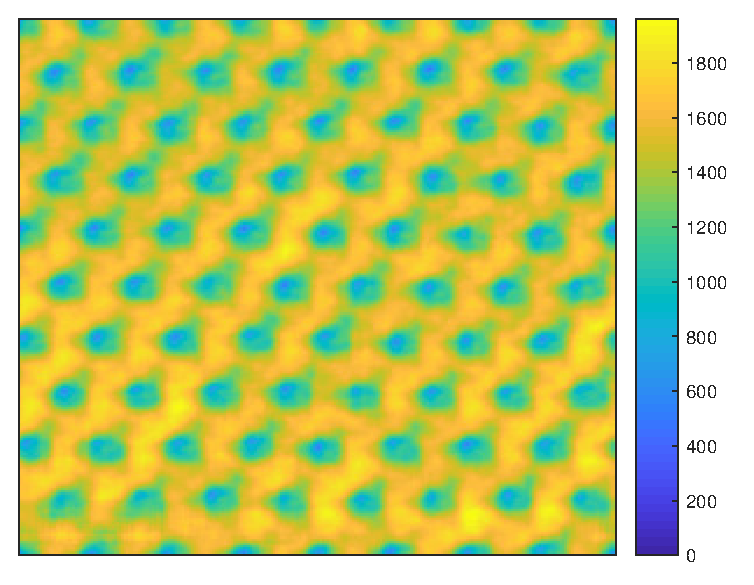
\includegraphics[width=.20\linewidth]{periodic_00_L2_20_superp_col.eps}} \hfill
  \subfloat{\includegraphics[width=.20\linewidth]{periodic_00_L1_20_superp_col.eps}} \hfill
  \subfloat{\includegraphics[width=.20\linewidth]{periodic_00_Linfinite_20_superp_col.eps}} \hfill
  \subfloat{\includegraphics[width=.20\linewidth]{periodic_00_ps_20_superp_col.eps}} \hfill
  \subfloat{\includegraphics[width=.20\linewidth]{periodic_00_cos_20_superp_col.eps}} \hfill \\
  \subfloat{\includegraphics[width=.18\linewidth]{stochastic_00_L2_20_superp.png}} \hfill
  \subfloat{\includegraphics[width=.18\linewidth]{stochastic_00_L1_20_superp.png}} \hfill
  \subfloat{\includegraphics[width=.18\linewidth]{stochastic_00_Linfinite_20_superp.png}} \hfill
  \subfloat{\includegraphics[width=.18\linewidth]{stochastic_00_ps_20_superp.png}} \hfill
  \subfloat{\includegraphics[width=.18\linewidth]{stochastic_00_cos_20_superp.png}} \hfill \\
  \subfloat[\s2]{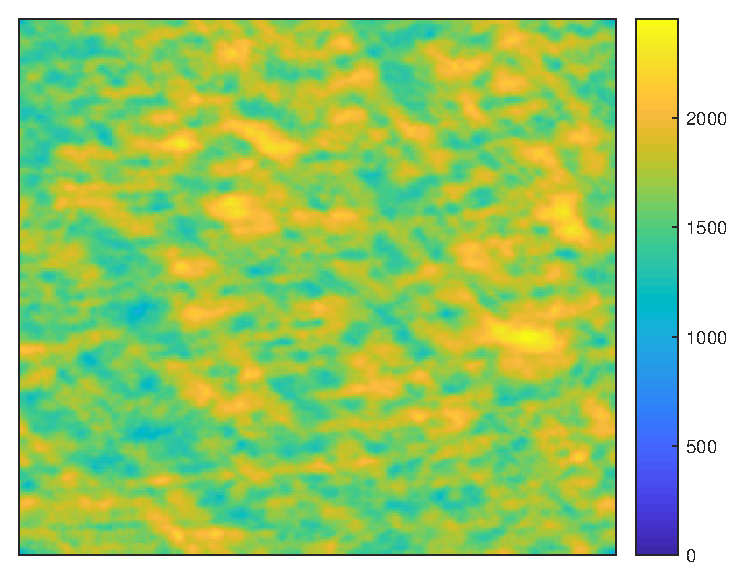
\includegraphics[width=.20\linewidth]{stochastic_00_L2_20_superp_col.eps}} \hfill
  \subfloat[\s1]{\includegraphics[width=.20\linewidth]{stochastic_00_L1_20_superp_col.eps}} \hfill
  \subfloat[\s{\infty}]{\includegraphics[width=.20\linewidth]{stochastic_00_Linfinite_20_superp_col.eps}} \hfill
  \subfloat[\sps]{\includegraphics[width=.20\linewidth]{stochastic_00_ps_20_superp_col.eps}} \hfill
  \subfloat[\scos]{\includegraphics[width=.20\linewidth]{stochastic_00_cos_20_superp_col.eps}} \hfill
  \caption{We select the upper-left patch in texture (b) in Figure \ref{fig:textures}. Here the selected patch is $20 \times 20$. We then compare this patch to all the other patches of the textures using different patch similarity function. The first twenty best matches are shown in red for all the different similarity functions considered (first row). We then compute the map of the patch similarity function for the upper-left patch and the periodic texture (second row). We observe that every similarity function detects patches that are perceptually similar to the original patch. Note also that in every case the most similar patch is the original one. Note also that even if here the patches are really similar the similarity functions do not choose the same patches. This first test can be considered as a sanity check. On the last two rows we conduct the same study on the stochastic texture. It is really interesting to note that in this case the Euclidean distance do not yield innovation. Indeed only two patches and their shifted versions for small shifts are selected. \s{\infty} \ yield a lot of different patches but a look at the similarity map indicate us that this similarity function is not likely to discriminate between patches. It can also be seen that the selected patches are not really similar to the original one. \s1 \ gives better results. \sps \ selects patches which have very similar structure to the original one but are brighter. This effect is reduced in \scos \ which also yields satisfactory results.}
  \label{fig:sim_func1}
\end{figure}
\begin{figure}[H]
  \centering
  \subfloat{\includegraphics[width=.18\linewidth]{periodic_00_L2_05_superp.png}} \hfill
  \subfloat{\includegraphics[width=.18\linewidth]{periodic_00_L1_05_superp.png}} \hfill
  \subfloat{\includegraphics[width=.18\linewidth]{periodic_00_Linfinite_05_superp.png}} \hfill
  \subfloat{\includegraphics[width=.18\linewidth]{periodic_00_ps_05_superp.png}} \hfill
  \subfloat{\includegraphics[width=.18\linewidth]{periodic_00_cos_05_superp.png}} \hfill \\
  \subfloat{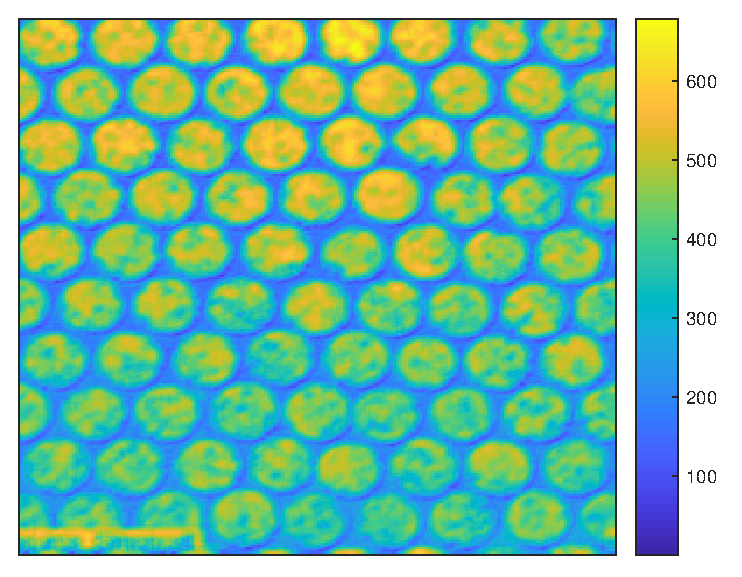
\includegraphics[width=.20\linewidth]{periodic_00_L2_05_superp_col.eps}} \hfill
  \subfloat{\includegraphics[width=.20\linewidth]{periodic_00_L1_05_superp_col.eps}} \hfill
  \subfloat{\includegraphics[width=.20\linewidth]{periodic_00_Linfinite_05_superp_col.eps}} \hfill
  \subfloat{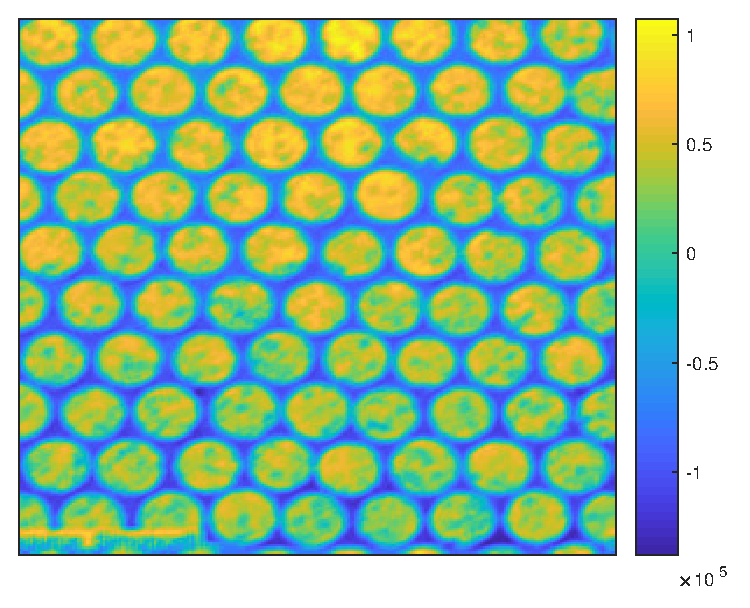
\includegraphics[width=.20\linewidth]{periodic_00_ps_05_superp_col.eps}} \hfill
  \subfloat{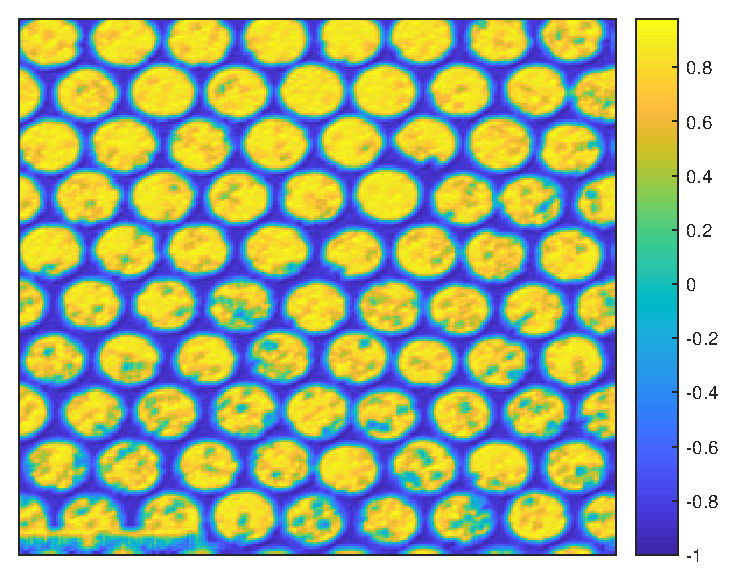
\includegraphics[width=.20\linewidth]{periodic_00_cos_05_superp_col.eps}} \hfill \\
    \subfloat{\includegraphics[width=.18\linewidth]{contrast_00_L2_20_superp.png}} \hfill
  \subfloat{\includegraphics[width=.18\linewidth]{contrast_00_L1_20_superp.png}} \hfill
  \subfloat{\includegraphics[width=.18\linewidth]{contrast_00_Linfinite_20_superp.png}} \hfill
  \subfloat{\includegraphics[width=.18\linewidth]{contrast_00_ps_20_superp.png}} \hfill
  \subfloat{\includegraphics[width=.18\linewidth]{contrast_00_cos_20_superp.png}} \hfill \\
  \subfloat[\s2]{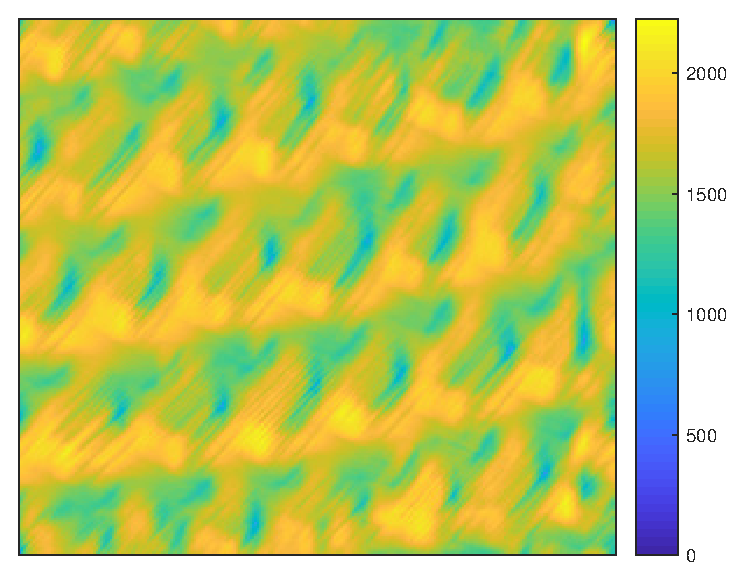
\includegraphics[width=.20\linewidth]{contrast_00_L2_20_superp_col.eps}} \hfill
  \subfloat[\s1]{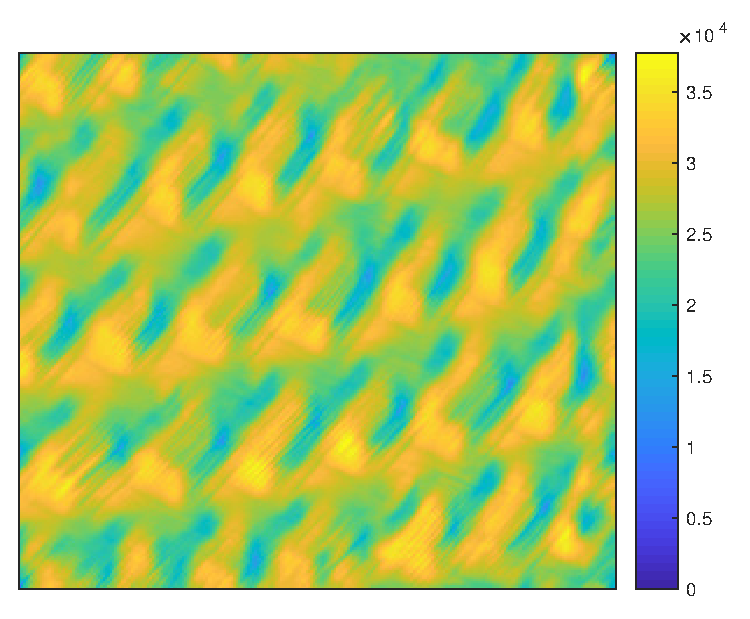
\includegraphics[width=.20\linewidth]{contrast_00_L1_20_superp_col.eps}} \hfill
  \subfloat[\s{\infty}]{\includegraphics[width=.20\linewidth]{contrast_00_Linfinite_20_superp_col.eps}} \hfill
  \subfloat[\sps]{\includegraphics[width=.20\linewidth]{contrast_00_ps_20_superp_col.eps}} \hfill
  \subfloat[\scos]{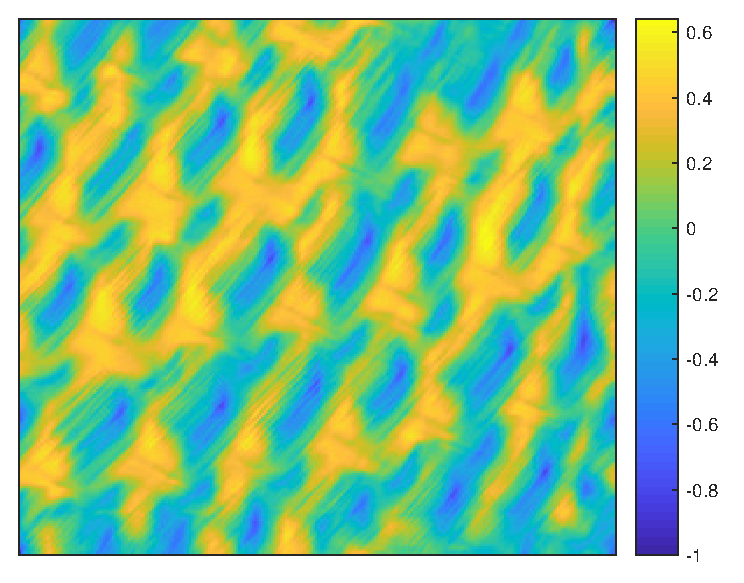
\includegraphics[width=.20\linewidth]{contrast_00_cos_20_superp_col.eps}} \hfill
  \caption{In this figure we reproduce the study conducted in the first row of Figure \ref{fig:sim_func1} but with a patch size of $5 \times 5$. In this cast the patch corresponds to an uniform zone. Every similarity function gives good perceptual results. However \sps \ fails to yield different patches. This is due to the fact \sps \ is sensible to the illumination of the scene. Thus here it will choose the darkest spot. Note that it makes no sense to consider \sps \ if the image has not been normalized as it will simply select the brightest patch. An interesting phenomenon occurs looking at the second row, the \scos \ similarity measure seems to be far more discriminative than the others. This effect could have been guessed in Figure \ref{fig:sim_func1} but is far more visible here. The last two rows reproduce the same study with patch size equals to $20 \times 20$ and original image being the texture with illumination defect. Once again \sps \ produces bad results since it focuses on the illumination more than the structure.}
  \label{fig:sim_func2}
\end{figure}
\begin{figure}[H]
  \subfloat{\includegraphics[width=.18\linewidth]{stochastic_00_L2_15_superp.png}} \hfill
  \subfloat{\includegraphics[width=.18\linewidth]{stochastic_00_L1_15_superp.png}} \hfill
  \subfloat{\includegraphics[width=.18\linewidth]{stochastic_00_Linfinite_15_superp.png}} \hfill
  \subfloat{\includegraphics[width=.18\linewidth]{stochastic_00_ps_15_superp.png}} \hfill
  \subfloat{\includegraphics[width=.18\linewidth]{stochastic_00_cos_15_superp.png}} \hfill \\
  \subfloat{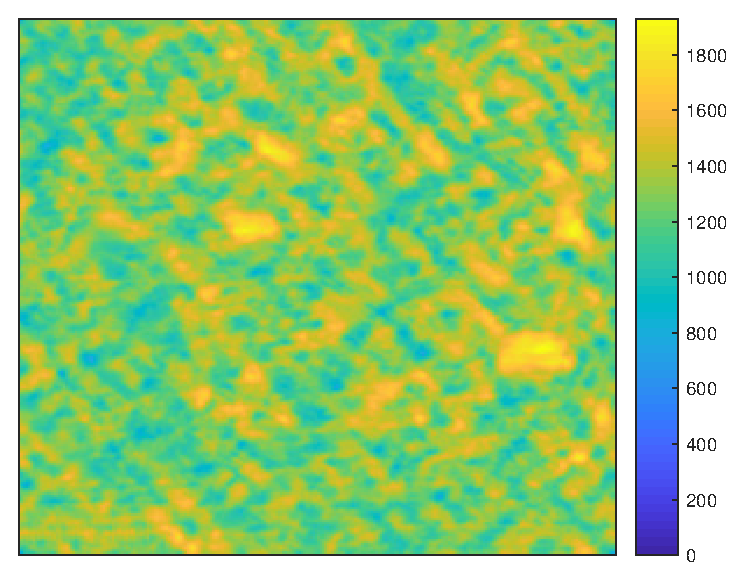
\includegraphics[width=.20\linewidth]{stochastic_00_L2_15_superp_col.eps}} \hfill
  \subfloat{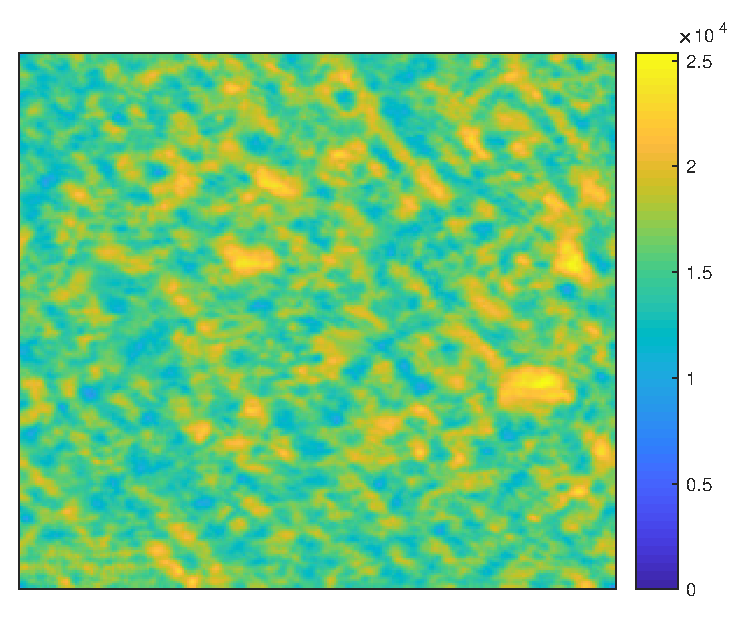
\includegraphics[width=.20\linewidth]{stochastic_00_L1_15_superp_col.eps}} \hfill
  \subfloat{\includegraphics[width=.20\linewidth]{stochastic_00_Linfinite_15_superp_col.eps}} \hfill
  \subfloat{\includegraphics[width=.20\linewidth]{stochastic_00_ps_15_superp_col.eps}} \hfill
  \subfloat{\includegraphics[width=.20\linewidth]{stochastic_00_cos_15_superp_col.eps}} \hfill \\
  \subfloat[\s2]{\includegraphics[width=.18\linewidth]{stochastic_00_L2_15_ecdf.eps}} \hfill
  \subfloat[\s1]{\includegraphics[width=.18\linewidth]{stochastic_00_L1_15_ecdf.eps}} \hfill
  \subfloat[\s{\infty}]{\includegraphics[width=.18\linewidth]{stochastic_00_Linfinite_15_ecdf.eps}} \hfill
  \subfloat[\sps]{\includegraphics[width=.18\linewidth]{stochastic_00_ps_15_ecdf.eps}} \hfill
  \subfloat[\scos]{\includegraphics[width=.18\linewidth]{stochastic_00_cos_15_ecdf.eps}} \hfill
  \caption{In this experiment we consider $15 \times 15$ patches and a stochastic texture. It is worth noticing that if \s{\infty} \ and \sps \ yield poor results, \s2 , \s1 and \scos \ give similar results. The positions identified using \scos \ and \s1 \ are also identified by \s2 . Note also that the similarity maps vary a lot depending on the similarity function. However, the empirical cumulative distribution function, c.d.f represented in the third row do not yield important information in order to identify the differences between these similarity functions.}
    \label{fig:sim_func3}
  \end{figure}
  \begin{figure}[H]
    \centering
    \raisebox{5em}{\rotatebox{90}{\s2}}
  \subfloat{\includegraphics[width=.25\linewidth]{contrast_00_L2_15_superp.png}} \hfill
  \subfloat{\includegraphics[width=.25\linewidth]{contrast_20_L2_15_superp.png}} \hfill
  \subfloat{\includegraphics[width=.25\linewidth]{contrast_50_L2_15_superp.png}} \hfill \\
    \raisebox{5em}{\rotatebox{90}{\s1}}
  \subfloat{\includegraphics[width=.25\linewidth]{contrast_00_L1_15_superp.png}} \hfill 
  \subfloat{\includegraphics[width=.25\linewidth]{contrast_20_L1_15_superp.png}} \hfill
  \subfloat{\includegraphics[width=.25\linewidth]{contrast_50_L1_15_superp.png}} \hfill \\
    \raisebox{5em}{\rotatebox{90}{\s{\infty}}}
  \subfloat{\includegraphics[width=.25\linewidth]{contrast_00_Linfinite_15_superp.png}} \hfill
  \subfloat{\includegraphics[width=.25\linewidth]{contrast_20_Linfinite_15_superp.png}} \hfill
  \subfloat{\includegraphics[width=.25\linewidth]{contrast_50_Linfinite_15_superp.png}} \hfill \\
    \raisebox{5em}{\rotatebox{90}{\scos}}
  \subfloat[$\sigma = 0$]{\includegraphics[width=.25\linewidth]{contrast_00_cos_15_superp.png}} \hfill
  \subfloat[$\sigma = 20$]{\includegraphics[width=.25\linewidth]{contrast_20_cos_15_superp.png}} \hfill
  \subfloat[$\sigma = 50$]{\includegraphics[width=.25\linewidth]{contrast_50_cos_15_superp.png}} \hfill \\
  \caption{In this figure we present the different results obtained for the four main relevant similarity functions for different additive white noise. $\sigma$ is the standard deviation of the additive white noise. For every similarity function adding noise yields more innovation in the process of selecting the best twenty patches. Here patch size is fixed to $\llbracket 1,15 \rrbracket \times \llbracket 1,15 \rrbracket$. Most of the time the new identified patches are perceptually acceptable.}
  \label{fig:noise_general}
\end{figure}
  \begin{figure}[H]
    \centering
    \raisebox{5em}{\rotatebox{90}{$\llbracket 1,10 \rrbracket^2$}}
  \subfloat{\includegraphics[width=.25\linewidth]{stochastic_00_L2_10_superp.png}} \hfill
  \subfloat{\includegraphics[width=.25\linewidth]{stochastic_20_L2_10_superp.png}} \hfill
  \subfloat{\includegraphics[width=.25\linewidth]{stochastic_50_L2_10_superp.png}} \hfill \\
    \raisebox{5em}{\rotatebox{90}{$\llbracket 1,15 \rrbracket^2$}}
  \subfloat{\includegraphics[width=.25\linewidth]{stochastic_00_L2_15_superp.png}} \hfill 
  \subfloat{\includegraphics[width=.25\linewidth]{stochastic_20_L2_15_superp.png}} \hfill
  \subfloat{\includegraphics[width=.25\linewidth]{stochastic_50_L2_15_superp.png}} \hfill \\
    \raisebox{5em}{\rotatebox{90}{$\llbracket 1,20 \rrbracket^2$}}
  \subfloat{\includegraphics[width=.25\linewidth]{stochastic_00_L2_20_superp.png}} \hfill
  \subfloat{\includegraphics[width=.25\linewidth]{stochastic_20_L2_20_superp.png}} \hfill
  \subfloat{\includegraphics[width=.25\linewidth]{stochastic_50_L2_20_superp.png}} \hfill \\
    \raisebox{5em}{\rotatebox{90}{$\llbracket 1,40 \rrbracket^2$}}
  \subfloat[$\sigma = 0$]{\includegraphics[width=.25\linewidth]{stochastic_00_L2_40_superp.png}} \hfill
  \subfloat[$\sigma =20$]{\includegraphics[width=.25\linewidth]{stochastic_20_L2_40_superp.png}} \hfill
  \subfloat[$\sigma = 50$]{\includegraphics[width=.25\linewidth]{stochastic_50_L2_40_superp.png}} \hfill \\
  \caption{In this figure we present the link between noise robustness and patch size in a stochastic texture. Here the study is presented for \s2 \ but the results would still be valid for any patch similarity function presented in Figure \ref{fig:noise_general}. The patch positions detected noisier image contained -subjects to certain outlets- the patch positions detected for smaller standard deviation. The set of the detected patch positions stabilized for a certain patch size. In our example for $\llbracket 1,20 \rrbracket^2$, there is only two patch positions detected for $\sigma = 20$ which are significantly different than the ones detected for $\sigma = 0$. However there are still many patches positions detected for $\sigma = 50$. The next patch size stabilizes every tested standard deviation.}
  \label{fig:noise_general}
\end{figure}


  \subparagraph{} We have seen in Figure \ref{fig:sim_func1} that the similarity functions gave satisfactory perceptual results. It is worth noticing, see Figure \ref{fig:sim_func2} that the results highly depend on the size of the patch. We also show that the \s1 \ and the \scos \ similarity function yield satisfactory perceptual results in Figure \ref{fig:sim_func3} even if \scos \ is not a distance. If the poor performance of the \sps \ similarity function was expected due to its sensibility to the illumination, the mild results of \s{\infty} \ are more surprising. No satisfying explanation was found to explain this type of behaviour. In the next section we present the results obtained when applying these functions to random fields.

  %}}}
%{{{ similarity functions and pdf

  \subsubsection{Similarity functions and p.d.f}
  In this section we will consider two cases:
  \begin{itemize}
  \item the white noise case where our spot in the \ADSN \ model will $\delta_0$,
  \item the full \ADSN \ model.
  \end{itemize}
  Our goal here is to confirm the results obtained in the previous section.
  We consider $\mathcal{P} = \llbracket 1,20 \rrbracket^2$ and $\Omega = \llbracket 1,512 \rrbracket^2$. We generate $N=1500$ \ADSN \ realizations. We consider the offset $(2,2)$ for the white noise and mild \ADSN \ model and $(10,20)$ for the full \ADSN . The choice of the offset is arbitrary.
  \begin{figure}[H]
    \centering
    \subfloat[white noise]{\includegraphics[width=0.24\linewidth]{white_noise.png}} \hfill
    \subfloat[mild \ADSN]{\includegraphics[width=0.24\linewidth]{mildADSN.png}} \hfill
    \subfloat[full \ADSN]{\includegraphics[width=0.24\linewidth]{fullADSN.png}} \\
    \subfloat{\includegraphics[width=0.24\linewidth]{white_noise_sample.png}} \hfill
    \subfloat{\includegraphics[width=0.24\linewidth]{mildADSN_sample.png}} \hfill
    \subfloat{\includegraphics[width=0.24\linewidth]{fullADSN_sample.png}} \hfill
    \caption{The spot is represented in the original domain $\Omega$. For example in the white noise the spot is only one white pixel in the upper-left corner. Same thing in the mild \ADSN \ which consists in a spot defined on $\llbracket 1,5 \rrbracket^2$ constant equals to one. The full \ADSN \ corresponds to a spot extracted from an image from the Simoncelli dataset. The spot is defined on $\llbracket 1,20\rrbracket^2$. On the second row we show one realization of the \ADSN \ model for each spot.}
    \label{fig:spot}    
  \end{figure}
    \begin{figure}[H]
    \centering
    \subfloat{\includegraphics[width=0.24\linewidth]{white_noise_offset_mat.png}} \hfill
    \subfloat{\includegraphics[width=0.24\linewidth]{mildADSN_offset_mat.png}} \hfill
    \subfloat{\includegraphics[width=0.24\linewidth]{fullADSN_offset_mat.png}} \\
    \subfloat[white noise]{\includegraphics[width=0.24\linewidth]{internal_l2_white_noise_20.eps}} \hfill
    \subfloat[mild \ADSN]{\includegraphics[width=0.24\linewidth]{internal_l2_mildADSN_20.eps}} \hfill
    \subfloat[full \ADSN]{\includegraphics[width=0.24\linewidth]{internal_l2_fullADSN_20.eps}} \hfill
    \caption{In this figure we show the offset correlation matrices for the different spots considered (first row). We also show the validity of Proposition \ref{p:s2internal} On each graph we represent the empirical c.d.f and the exact c.d.f computed with the Imhof integral.}
    \label{fig:l2}    
  \end{figure}
  \begin{figure}[H]
    \raisebox{2ex}{\rotatebox{90}{internal - scalar product}}
    \subfloat{\includegraphics[width=0.32\linewidth]{internal_ps_white_noise_20.eps}} \hfill
    \subfloat{\includegraphics[width=0.32\linewidth]{internal_ps_mildADSN_20.eps}} \hfill
    \subfloat{\includegraphics[width=0.32\linewidth]{internal_ps_fullADSN_20.eps}} \\
    \raisebox{5ex}{\rotatebox{90}{internal - cosine}}    
    \subfloat{\includegraphics[width=0.32\linewidth]{internal_cos_white_noise_20.eps}} \hfill
    \subfloat{\includegraphics[width=0.32\linewidth]{internal_cos_mildADSN_20.eps}} \hfill
    \subfloat{\includegraphics[width=0.32\linewidth]{internal_cos_fullADSN_20.eps}} \\
    \raisebox{2ex}{\rotatebox{90}{template - scalar product}}    
    \subfloat{\includegraphics[width=0.32\linewidth]{template_ps_white_noise_20.eps}} \hfill
    \subfloat{\includegraphics[width=0.32\linewidth]{template_ps_mildADSN_20.eps}} \hfill
    \subfloat{\includegraphics[width=0.32\linewidth]{template_ps_fullADSN_20.eps}} \\
    \raisebox{5ex}{\rotatebox{90}{template - cosine}}    
    \subfloat[white noise]{\includegraphics[width=0.32\linewidth]{template_cos_white_noise_20.eps}} \hfill
    \subfloat[mild \ADSN]{\includegraphics[width=0.32\linewidth]{template_cos_mildADSN_20.eps}} \hfill
    \subfloat[full \ADSN]{\includegraphics[width=0.32\linewidth]{template_cos_fullADSN_20.eps}} \hfill
    \caption{In this figure we illustrate the convergence in law announced in Propositions \ref{p:spsinternal}, \ref{p:spstemplate}, \ref{p:scosinternal}, \ref{p:scostemplate}. First row corresponds to \internalmatching \ and scalar product, i.e Proposition \ref{p:spsinternal} Second row corresponds to \internalmatching \ and cosine, i.e Proposition \ref{p:scosinternal} Third row corresponds to \templatematching \ and scalar product, i.e Proposition \ref{p:spstemplate} Fourth row corresponds to \templatematching \ and cosine, i.e Proposition \ref{p:spsinternal}}
    \label{fig:tcl}
    \end{figure}

    %}}}
%{{{ internal experiments optimal NFA

\subsubsection{Optimal NFA}
\label{sec:optimal_nfa}
We now proceed to the comparison of patch similarity functions.
First let us recall a few things about the \NFA. 
\TODO{rappeler les choses sur l'optimalité}
We face two problems here:
\begin{itemize}
\item we set the \NFA \ pixel-wise. Thus we know that theoretically the number of detection in the \acontrario \ model is 
  less than the \NFA . But we do not know what is the true \NFA . In usual settings, since we have independence between
  our experiments we can state that the \NFA \ is simply the number of experiments time the parameter $a$. But in our case,
  an experiment is the comparison of two patches and two patches can be highly correlated,
\item we are working in an asymptotic case. In an exact setting, this problem does not occur. However when we suppose that
  we have reached the asymptotic mode two strong assumptions are made :
  \begin{enumerate}
  \item the distribution of the patch similarity function is Gaussian,
    \item the mean and the variance of the patch similarity function are the ones computed theoretically.
      \end{enumerate}
      We will see that the Gaussian assumption is not well suited for some patch similarity functions and even if the Gaussian
      distribution seems to fit the empirical p.d.f, visual clues may not be of interest. Indeed we are looking for very low
      values of the c.d.f. Hence if the histogram and the true p.d.f match near the mean it does not necessarily means that this
      property holds for the queue of the distribution.
    \end{itemize}


    \begin{table}[H]
      \centering
   \caption{Internal asymptotic square Euclidean \NFA}      
 \begin{tabular}{|c||c|c|c|c|c|c|c|c|}
 \hline 
\diagbox{spot size }{patch size} & 5    & 10   & 15   & 20   & 30   & 40   & 50   & 70   \\ \hline \hline 
1                                & 0.33 & 1.38 & 3.19 & 4.56 & 6.53 & 7.37 & 8.18 & 8.97 \\ \hline 
2                                & 0.34 & 0.39 & 1.19 & 2.19 & 4.43 & 5.80 & 6.64 & 8.51 \\ \hline 
5                                & 0.35 & 0.39 & 0.44 & 0.49 & 0.63 & 1.29 & 2.31 & 4.07 \\ \hline 
10                               &      & 0.40 & 0.45 & 0.49 & 0.47 & 0.44 & 0.51 & 1.43 \\ \hline 
15                               &      &      & 0.45 & 0.48 & 0.47 & 0.45 & 0.48 & 0.53 \\ \hline 
20                               &      &      &      & 0.52 & 0.50 & 0.47 & 0.48 & 0.49 \\ \hline 
25                               &      &      &      &      & 0.49 & 0.48 & 0.50 & 0.49 \\ \hline 
 \end{tabular}
 \caption*{Number of detections with different patch sizes and spot sizes for the $L^2$ patch similarity function with asymptotic p.d.f. \NFA \ was set to ten. $5000$ \ADSN \ images were generated for each setting. The number in each cell of the table is the mean of the number of detection corresponding to the asymptotic $L^2$ patch similarity setting with $\operatorname{NFA} = 10$. The generated images are squared with width $128$ pixels.}
 \label{t:internal_ADSN_res_L2}
 \end{table}
 \begin{table}[H]
   \centering
   \caption{Internal scalar product matching \NFA}
 \begin{tabular}{|c||c|c|c|c|c|c|c|c|}
 \hline 
\diagbox{spot size }{patch size} & 5     & 10    & 15    & 20    & 30    & 40    & 50    & 70    \\ \hline \hline 
1                                & 18.09 & 11.63 & 10.89 & 10.44 & 10.15 & 10.07 & 9.97  & 10.04 \\ \hline 
2                                & 34.17 & 16.52 & 12.76 & 11.54 & 10.59 & 10.38 & 10.27 & 9.90  \\ \hline 
5                                & 93.93 & 49.30 & 30.82 & 20.90 & 15.32 & 13.18 & 12.12 & 11.51 \\ \hline 
10                               &       & 86.68 & 57.59 & 45.97 & 28.17 & 19.65 & 17.35 & 14.54 \\ \hline 
15                               &       &       & 83.93 & 63.81 & 43.07 & 29.97 & 25.66 & 18.23 \\ \hline 
20                               &       &       &       & 79.45 & 52.81 & 36.69 & 33.24 & 24.74 \\ \hline 
25                               &       &       &       &       & 68.27 & 51.49 & 40.26 & 26.60 \\ \hline 
 \end{tabular}
 \caption*{Number of detections with different patch sizes and spot sizes for the scalar product patch similarity function with asymptotic p.d.f. \NFA \ was set to ten. $5000$ \ADSN \ images were generated for each setting. The number in each cell of the table is the mean of the number of detection corresponding to the asymptotic scalar product patch similarity setting with $\operatorname{NFA} = 10$. The generated images are squared with width $128$ pixels.}
 \label{t:internal_ADSN_res_ps}
 \end{table}

 \begin{table}[H]
   \centering
   \caption{Internal cosine matching \NFA}
 \begin{tabular}{|c||c|c|c|c|c|c|c|c|}
 \hline 
\diagbox{spot size }{patch size} & 5    & 10   & 15   & 20   & 30   & 40   & 50   & 70    \\ \hline \hline 
1                                & 3.08 & 8.10 & 9.11 & 9.61 & 9.89 & 9.92 & 9.94 & 10.00 \\ \hline 
2                                & 0.04 & 5.01 & 7.54 & 8.56 & 9.38 & 9.79 & 9.73 & 10.00 \\ \hline 
5                                & 0.00 & 0.00 & 1.36 & 3.85 & 6.95 & 8.25 & 8.88 & 9.58  \\ \hline 
10                               &      & 0.00 & 0.00 & 0.00 & 1.77 & 4.25 & 6.25 & 7.89  \\ \hline 
15                               &      &      & 0.00 & 0.00 & 0.01 & 0.92 & 2.66 & 6.36  \\ \hline 
20                               &      &      &      & 0.00 & 0.00 & 0.00 & 0.61 & 3.60  \\ \hline 
25                               &      &      &      &      & 0.00 & 0.00 & 0.01 & 2.24  \\ \hline 
 \end{tabular}
 \caption*{Number of detections with different patch sizes and spot sizes for the cosine patch similarity function with asymptotic p.d.f. \NFA \ was set to ten. $5000$ \ADSN \ images were generated for each setting. The number in each cell of the table is the mean of the number of detection corresponding to the asymptotic cosine patch similarity setting with $\operatorname{NFA} = 10$. The generated images are squared with width $128$ pixels.}
 \label{t:internal_ADSN_res_cos}
\end{table}

    \begin{table}[H]
      \centering
      \caption{Template asymptotic square Euclidean \NFA}
       \begin{tabular}{|c||c|c|c|c|c|c|c|c|}
 \hline 
\diagbox{spot size }{patch size} & 5    & 10   & 15   & 20   & 30   & 40   & 50   & 70   \\ \hline \hline 
1                                & 0.00 & 1.53 & 3.81 & 5.11 & 6.40 & 7.83 & 7.74 & 9.26 \\ \hline 
2                                & 0.00 & 0.00 & 0.32 & 1.24 & 3.16 & 4.51 & 5.41 & 7.69 \\ \hline 
5                                & 0.00 & 0.00 & 0.00 & 0.00 & 0.02 & 0.42 & 1.43 & 2.99 \\ \hline 
10                               &      & 0.00 & 0.00 & 0.00 & 0.00 & 0.00 & 0.00 & 0.37 \\ \hline 
15                               &      &      & 0.00 & 0.00 & 0.00 & 0.00 & 0.00 & 0.02 \\ \hline 
20                               &      &      &      & 0.00 & 0.00 & 0.00 & 0.00 & 0.00 \\ \hline 
25                               &      &      &      &      & 0.00 & 0.00 & 0.00 & 0.00 \\ \hline 
\end{tabular} 
 \caption*{Number of detections with different patch sizes and spot sizes for the $L^2$ patch similarity function with asymptotic p.d.f. \NFA \ was set to ten. $5000$ \ADSN \ images were generated for each setting. The number in each cell of the table is the mean of the number of detection corresponding to the asymptotic $L^2$ patch similarity setting with $\operatorname{NFA} = 10$. The generated images are squared with width $128$ pixels.}
 \label{t:template_ADSN_res_L2}
 \end{table}
 \begin{table}[H]
   \centering
   \caption{Template scalar product matching \NFA}
      \begin{tabular}{|c||c|c|c|c|c|c|c|c|}
 \hline 
\diagbox{spot size }{patch size} & 5     & 10    & 15    & 20    & 30    & 40    & 50    & 70    \\ \hline \hline 
1                                & 10.01 & 10.06 & 10.01 & 10.09 & 9.97  & 10.50 & 9.24  & 10.60 \\ \hline 
2                                & 10.10 & 9.85  & 10.11 & 9.93  & 10.05 & 10.28 & 10.66 & 9.95  \\ \hline 
5                                & 9.93  & 10.57 & 10.02 & 9.83  & 9.58  & 10.13 & 10.08 & 11.93 \\ \hline 
10                               &       & 9.69  & 10.33 & 9.25  & 9.99  & 9.75  & 9.04  & 10.46 \\ \hline 
15                               &       &       & 9.28  & 9.40  & 10.33 & 8.75  & 9.70  & 11.37 \\ \hline 
20                               &       &       &       & 9.60  & 10.44 & 12.12 & 10.61 & 10.95 \\ \hline 
25                               &       &       &       &       & 9.49  & 11.30 & 10.46 & 8.96  \\ \hline 
\end{tabular} 
 \caption*{Number of detections with different patch sizes and spot sizes for the scalar product patch similarity function with asymptotic p.d.f. \NFA \ was set to ten. $5000$ \ADSN \ images were generated for each setting. The number in each cell of the table is the mean of the number of detection corresponding to the asymptotic scalar product patch similarity setting with $\operatorname{NFA} = 10$. The generated images are squared with width $128$ pixels.}
 \label{t:template_ADSN_res_ps}
 \end{table}

 \begin{table}[H]
   \centering
   \caption{Template cosine matching \NFA}
   \begin{tabular}{|c||c|c|c|c|c|c|c|c|}
 \hline 
\diagbox{spot size }{patch size} & 5    & 10   & 15   & 20   & 30   & 40   & 50    & 70   \\ \hline \hline 
1                                & 3.04 & 8.22 & 9.09 & 9.88 & 9.63 & 9.64 & 10.23 & 9.42 \\ \hline 
2                                & 0.00 & 2.14 & 5.83 & 8.02 & 8.40 & 9.66 & 8.88  & 8.52 \\ \hline 
5                                & 0.00 & 0.00 & 0.00 & 0.47 & 3.77 & 6.71 & 7.27  & 8.67 \\ \hline 
10                               &      & 0.00 & 0.00 & 0.00 & 0.00 & 0.90 & 3.80  & 6.14 \\ \hline 
15                               &      &      & 0.00 & 0.00 & 0.00 & 0.00 & 0.28  & 3.75 \\ \hline 
20                               &      &      &      & 0.00 & 0.00 & 0.00 & 0.00  & 1.32 \\ \hline 
25                               &      &      &      &      & 0.00 & 0.00 & 0.00  & 0.08 \\ \hline 
\end{tabular} 
 \caption*{Number of detections with different patch sizes and spot sizes for the cosine patch similarity function with asymptotic p.d.f. \NFA \ was set to ten. $5000$ \ADSN \ images were generated for each setting. The number in each cell of the table is the mean of the number of detection corresponding to the asymptotic cosine patch similarity setting with $\operatorname{NFA} = 10$. The generated images are squared with width $128$ pixels.}
 \label{t:template_ADSN_res_cos}
 \end{table}

 Results are summarized in tables \ref{t:internal_ADSN_res_L2}, \ref{t:internal_ADSN_res_ps}, \ref{t:internal_ADSN_res_cos}, \ref{t:template_ADSN_res_L2}, \ref{t:template_ADSN_res_ps}, \ref{t:template_ADSN_res_cos}. The internal matching and the template matching cases were investigated and the \NFA \ was set to ten. Three different asymptotic methods were used:
 \begin{itemize}
 \item asymptotic $L^2$,
 \item asymptotic scalar product,
 \item asymptotic cosine.
 \end{itemize}
 For each function we computed the number of detections in the case of the spot size was less than the patch size. This is a clear restriction compared to the exact case where every spot size was allowed. Indeed if the spot size is larger than the patch size there is little hope for us to be in what we called an asymptotic case. In the template matching the template was set to be a patch of the original image from which the \ADSN \ spot was extracted. The size of the template was set to be the one of the patch size.
 \subparagraph{Interpretation} We study two settings, the internal matching and the template matching. In both cases square Euclidean, scalar product and cosine similarity functions and the robustness of their asymptotic behavior is investigated:
 \begin{itemize}
 \item internal matching: looking at tables \ref{t:internal_ADSN_res_L2}, \ref{t:internal_ADSN_res_ps}, \ref{t:internal_ADSN_res_cos}, $L^2$ and cosine patch similarity functions yield less detections than the \NFA . This effect is clear when looking at a patch size equals to the spot size. An explanation is that we are far from the asymptotic case, i.e the data is still highly correlated. The effect is reverse for the scalar product but the explanation remains the same. The cosine function has a better behavior than the asymptotic $L^2$ function. One explanation may be that the normality is a better hypothesis for the cosine function than for the $L^2$ function, see Figure \ref{fig:isgaussian_internal}.
 \item template matching: looking at tables \ref{t:template_ADSN_res_L2}, \ref{t:template_ADSN_res_ps}, \ref{t:template_ADSN_res_cos}, $L^2$ and cosine patch similarity functions yield less detections than the \NFA . This result was already noted in the internal case. Once again, the asymptotic case for the cosine function seems more robust. The best, and ideal, behavior is obtained for the scalar product. Indeed, in the scalar product case the asymptotic case is in fact exact. Thus, the number of detections is higher. Note that even if for each offset the Gaussian assumption is true this does not mean that the expected number of detections should be equal to the \NFA . Indeed, there is still no independence assumptions between the offsets.
 \end{itemize}
 This study highlights two important points. First of all, when dealing with asymptotic patch similarity function one must consider models in which there is no very long space correlation, the robustness of the patch similarity function to this space correlation varies. Secondly, the \NFA , i.e the Number of False Alarms which is defined to be the number of experiments time a parameter, \textbf{is not} equal to the expected number of detection even in the ideal case since there is no independence between the offsets. However, this \NFA is an upper bound to the expected number of detections. These results seem to rule out the asymptotic patch similarity functions since we are bound to restrictive cases of \ADSN \ models but we underline the fact that even with a small spot an \ADSN \ still gives spatial information and is more discriminative than a white noise. An other interest of asymptotic methods are their speed. Indeed, using convolution properties and the \FFT \ implementation we can build c.d.f maps very fast. In the next section we evaluate the \acontrario \ detections using these asymptotic detection functions.
  \begin{figure}[H]
    \centering
    \subfloat[square Euclidean]{\includegraphics[width=0.33\linewidth]{isgaussian_internal_L2_10_10.eps}} \hfill
    \subfloat[scalar product]{\includegraphics[width=0.33\linewidth]{isgaussian_internal_ps_10_10.eps}} \hfill
    \subfloat[cosine]{\includegraphics[width=0.33\linewidth]{isgaussian_internal_cos_10_10.eps}}     
    \caption{Empirical distribution function of different similarity functions for offset $(10,10)$, patch size of ten pixels, spot size of ten pixels in an internal matching setting. The empirical distribution function was computed on $1000$ \ADSN \ models. Since we are in a limit case the empirical p.d.f is clearly not Gaussian. However the order two statistics of the empirical distribution are well estimated. For example the $L^1$ norm of the empirical mean of the centered and normalized data for $10000$ \ADSN \ models is $0.0117$ in the square Euclidean asymptotic case, $0.0138$ in the scalar product case, $0.0125$ in the cosine case. For the same data, the $L^1$ distance between the empirical standard deviation and $1$ is $0.0114$ in the square Euclidean asymptotic case, $0.0189$ in the scalar product case, $0.1757$ in the cosine case.}
    \label{fig:isgaussian_internal}    
  \end{figure}

%}}}
%{{{ perceptual criterion and a contrario detection

\subsubsection{Perceptual criterion and \acontrario \ detection}
% plan : on va évaluer sur la très régulière. On ne traite que le cadre internal ici (justification :
% car on est dans une situation d'illustration). Dans le cas de l'asymptotique on sait ce que l'on veut
% découvrir = bon ``checking''. Après dans d'autres images c'est plus compliqué...
% Trouver une image très géométrique pour voir si des structures sont repérées (aspect Gestalt = bof on
% est plus sur de l'info texturée)
% Ajouter du bruit des structures randoms
% étudier l'influence de prendre les minima
\subparagraph{Introduction}
% on va présenter diverses xps. D'abord sur une texture très régulière pour vérifier (safety check).
% On teste avec différents modèles, différents NFA.
% on va ajouter du bruit. On va ensuite tester pour des choses sur lesquelles ce n'est pas clair
% quelle structure doit être détectée.
% Importance de choisir les minima. Ici on introduit ces idées : mettre en avant que l'on ne sait
% pas vraiment ce que l'on cherche (pas de fonction d'évaluation).
In this section we implement the \acontrario \ model using the asymptotic patch similarity functions. Our goal is to investigate the results on a perceptual point of view. A first study on the influence of
the patch similarity function on the perceptual discrimination was given in Section \ref{s:a_perceptual_study}, but this study was conducted on procedures which were not part of an \acontrario \ framework (ranking, thresholding). We now derive an \acontrario \ model in the asymptotic case. Every time we compare the different asymptotic patch similarity functions. First we study the influence of the choice of the \ADSN \ model and the \NFA \ settings. We then study the influence of the noise in the image and finally give a minima selection procedure which allows us to work with sparser images.
\subparagraph{\ADSN \ models and \NFA \ study}
We have seen in the previous Section that the size of the spot greatly influences the performance of the \acontrario \ detection and its accuracy. It is then natural to ask ourselves how to set the spot in the \ADSN \ model in an \acontrario \ model. Let us fix some notations. Let $X_0$ be the original image. Let $n_h \in \N$ be the size of the spot. We suppose the mean of $X_0$ is zero, i.e $m(X_0) = 0$ and that its standard deviation is one, i.e $\sigma(X_0) = 1$. We define the spot $h$ to be the restriction of $X_0$ to $\llbracket 0,n_h \rrbracket^2$. Setting the spot in this manner the \ADSN \ realizations will have different different mean and standard deviation than the original image. In order to obtain a microtexture model which has the same order one and two statistics as the original image we center $h$ and divide $h$ by its squared Euclidean norm. Thus, the \ADSN \ realizations using this spot will have same empirical mean and variance \textbf{in expectation}.
\comment{(13/12/17) On ne prend pas en compte les problèmes de périodicité... On devrait aussi peut-être considérer
  un modèle représentant la microtexture global dans un petit patch plutôt que de procéder à une crop qui
  peut s'avérer peu judicieux.}
In the following study we test the following values for the parameters:
\begin{itemize}
\item spot size: $1$, $5$, $10$, $20$ and $100$ pixels (in a $256 \times 256$ image),
\item \NFA : $1$, $10$, $50$,
\item $\sigma$ : $1$, $10$, $20$, $50$ (standard deviation of a Gaussian noise added to the image as preprocessing).
\end{itemize}
Every image tested here was extracted from the Simoncelli dataset and originally takes its values between $0$ and $255$ (gray levels). In every result presented here one last step was added, instead of performing the detection on all the offsets we only the consider the ones that represent local minima of the c.d.f according to the 8-connexity. Doing so we greatly reduce the number of detections and obtain sparse figures, see Figure \ref{f:minima_justif} for an illustration. In what follows we are going to present four results:
\begin{itemize}
\item \textbf{Robustness to noise:} in Figure \ref{f:robustness_noise} we present results about the robustness of the \acontrario \ methods when we add noise to the original image. Our conclusion will be that the detection is robust. However we identify that the more periodic the texture the more robust the detection,
\item \textbf{Model size:} the size of the spot may be the most limitant factor of our study. Indeed, the number of detections greatly depends on the size of the spot. This situation and explanations are provided in Figure \ref{f:model_size},
\item \textbf{Similarity functions comparison:} in Figure \ref{f:robustness_detection} we compare the number and the locations of the detections of the three investigated similarity functions. Different settings, i.e different textures, lead to different results.
\item \textbf{Perceptual questions:} in some situations, presented in Figure \ref{f:perceptual_question}, it is difficult to assert if there is indeed a similar patch in the image. These results underline the need for a satisfying measure of perceptual similarity in patch comparison.
\end{itemize}
\captionsetup[subfigure]{labelformat=parens}
\begin{figure}[H]
  \centering
  {\includegraphics[width=.24\linewidth]{18/percep_thres_01_cos_010_01.png}} \hfill
  {\includegraphics[width=.24\linewidth]{18/percep_thres_01_cos_020_01.png}} \hfill
  {\includegraphics[width=.24\linewidth]{18/percep_minthres_01_cos_010_01.png}} \hfill
  {\includegraphics[width=.24\linewidth]{18/percep_minthres_01_cos_020_01.png}} \hfill \\
  \subfloat[]{\includegraphics[width=.24\linewidth]{06/percep_thres_01_cos_010_01.png}} \hfill
  \subfloat[]{\includegraphics[width=.24\linewidth]{06/percep_thres_01_cos_020_01.png}} \hfill
  \subfloat[]{\includegraphics[width=.24\linewidth]{06/percep_minthres_01_cos_010_01.png}} \hfill
  \subfloat[]{\includegraphics[width=.24\linewidth]{06/percep_minthres_01_cos_020_01.png}} \hfill  
  \caption{Each row corresponds to several detections on different periodic texture images. In each image we are looking for patch similar to the upper left patch (green box). The identified patches using a \NFA \ of one, the cosine similarity function and a spot size of ten pixels (a) or twenty pixels (b) are displayed in red boxes. The same study is conducted on local minima of the c.d.f map only (c) and (d). It is clear that the figures presented in (c) and (d) are sparser than their equivalent in columns (a) and (b). The results presented here are also valid for other spot sizes and similarity functions.}
  \label{f:minima_justif}
\end{figure}
\captionsetup[subfigure]{labelformat=empty}
\begin{figure}[H]
  \centering
  {\includegraphics[width=.24\linewidth]{18/percep_minthres_01_cos_010_01.png}} \hfill
  {\includegraphics[width=.24\linewidth]{18/percep_minthres_01_cos_010_10.png}} \hfill
  {\includegraphics[width=.24\linewidth]{18/percep_minthres_01_cos_010_20.png}} \hfill  
  {\includegraphics[width=.24\linewidth]{18/percep_minthres_01_cos_010_50.png}} \hfill \\
  {\includegraphics[width=.24\linewidth]{03/percep_minthres_01_cos_010_01.png}} \hfill
  {\includegraphics[width=.24\linewidth]{03/percep_minthres_01_cos_010_10.png}} \hfill
  {\includegraphics[width=.24\linewidth]{03/percep_minthres_01_cos_010_20.png}} \hfill  
  {\includegraphics[width=.24\linewidth]{03/percep_minthres_01_cos_010_50.png}} \hfill \\
  \subfloat[$\sigma=1$]{\includegraphics[width=.24\linewidth]{02/percep_minthres_01_cos_010_01.png}} \hfill
  \subfloat[$\sigma=10$]{\includegraphics[width=.24\linewidth]{02/percep_minthres_01_cos_010_10.png}} \hfill
  \subfloat[$\sigma=20$]{\includegraphics[width=.24\linewidth]{02/percep_minthres_01_cos_010_20.png}} \hfill  
  \subfloat[$\sigma=50$]{\includegraphics[width=.24\linewidth]{02/percep_minthres_01_cos_010_50.png}} \hfill \\
  \caption{Each row corresponds to several detections on different periodic texture images. In each image we are looking for patch similar to the upper left patch (green box). The identified patches using a \NFA \ of one, the cosine similarity function and a spot size of ten pixels. Each column corresponds to the detections obtained under a random Gaussian noise. The image and the detections are presented without the noise here (however the detection is performed on the noisy images). There is little to no change to the detections made, a careful flip could show that some of the boxes are displaced from a few pixels.The last row shows a little more variability. This could be explained by the fact that high frequencies are destroyed when adding noise. The results presented here are also for other spot sizes and similarity functions.}
  \label{f:robustness_noise}
\end{figure}
\begin{figure}[H]
  \centering
  {\includegraphics[width=.24\linewidth]{01/percep_minthres_01_cos_001_00.png}} \hfill
  {\includegraphics[width=.24\linewidth]{01/percep_minthres_01_cos_005_00.png}} \hfill
  {\includegraphics[width=.24\linewidth]{01/percep_minthres_01_cos_010_00.png}} \hfill  
  {\includegraphics[width=.24\linewidth]{01/percep_minthres_01_cos_020_00.png}} \hfill \\
  {\includegraphics[width=.24\linewidth]{05/percep_minthres_01_cos_001_00.png}} \hfill
  {\includegraphics[width=.24\linewidth]{05/percep_minthres_01_cos_005_00.png}} \hfill
  {\includegraphics[width=.24\linewidth]{05/percep_minthres_01_cos_010_00.png}} \hfill  
  {\includegraphics[width=.24\linewidth]{05/percep_minthres_01_cos_020_00.png}} \hfill \\
  {\includegraphics[width=.24\linewidth]{17/percep_minthres_01_cos_001_00.png}} \hfill
  {\includegraphics[width=.24\linewidth]{17/percep_minthres_01_cos_005_00.png}} \hfill
  {\includegraphics[width=.24\linewidth]{17/percep_minthres_01_cos_010_00.png}} \hfill  
  {\includegraphics[width=.24\linewidth]{17/percep_minthres_01_cos_020_00.png}} \hfill \\
  \subfloat[$n_h=1$]{\includegraphics[width=.24\linewidth]{16/percep_minthres_01_cos_001_00.png}} \hfill
  \subfloat[$n_h=5$]{\includegraphics[width=.24\linewidth]{16/percep_minthres_01_cos_005_00.png}} \hfill
  \subfloat[$n_h=10$]{\includegraphics[width=.24\linewidth]{16/percep_minthres_01_cos_010_00.png}} \hfill  
  \subfloat[$n_h=20$]{\includegraphics[width=.24\linewidth]{16/percep_minthres_01_cos_020_00.png}} \hfill \\
  \caption{Each row corresponds to several detections on different periodic texture images. In each image we are looking for patch similar to the upper left patch (green box). The identified patches using a \NFA \ of one, the cosine similarity function. No noise was added. Each column corresponds to a different spot size; The number of detections clearly decrease no matter if the texture is stochastic or periodic. Two explanations can be formulated to explain this problem. First of all, a white noise model is not sufficient to explain the micro texture image thus yielding to many detections. Moreover, when looking at large spot sizes the asymptotic behaviour is far from being reached (as highlighted in Section \ref{sec:optimal_nfa} and Tables \ref{t:internal_ADSN_res_L2}, \ref{t:internal_ADSN_res_ps}, \ref{t:internal_ADSN_res_cos}. These results remain true for other similarity functions. In figure \ref{f:robustness_detection} we investigate the robustness of these similarity functions.}
  \label{f:model_size}
\end{figure}

\begin{figure}[H]
  \centering
  {\includegraphics[width=.24\linewidth]{04/percep_minthres_01_ps_001_00.png}} \hfill
  {\includegraphics[width=.24\linewidth]{04/percep_minthres_01_ps_005_00.png}} \hfill
  {\includegraphics[width=.24\linewidth]{04/percep_minthres_01_ps_010_00.png}} \hfill  
  {\includegraphics[width=.24\linewidth]{04/percep_minthres_01_ps_020_00.png}} \hfill \\
  {\includegraphics[width=.24\linewidth]{04/percep_minthres_01_cos_001_00.png}} \hfill
  {\includegraphics[width=.24\linewidth]{04/percep_minthres_01_cos_005_00.png}} \hfill
  {\includegraphics[width=.24\linewidth]{04/percep_minthres_01_cos_010_00.png}} \hfill  
  {\includegraphics[width=.24\linewidth]{04/percep_minthres_01_cos_020_00.png}} \hfill \\  
  {\includegraphics[width=.24\linewidth]{04/percep_minthres_01_L2asymp_001_00.png}} \hfill
  {\includegraphics[width=.24\linewidth]{04/percep_minthres_01_L2asymp_005_00.png}} \hfill
  {\includegraphics[width=.24\linewidth]{04/percep_minthres_01_L2asymp_010_00.png}} \hfill  
  {\includegraphics[width=.24\linewidth]{04/percep_minthres_01_L2asymp_020_00.png}} \hfill \\
  {\includegraphics[width=.24\linewidth]{15/percep_minthres_01_cos_001_00.png}} \hfill
  {\includegraphics[width=.24\linewidth]{15/percep_minthres_01_cos_005_00.png}} \hfill
  {\includegraphics[width=.24\linewidth]{15/percep_minthres_01_cos_010_00.png}} \hfill  
  {\includegraphics[width=.24\linewidth]{15/percep_minthres_01_cos_020_00.png}} \hfill \\
  {\includegraphics[width=.24\linewidth]{15/percep_minthres_01_ps_001_00.png}} \hfill
  {\includegraphics[width=.24\linewidth]{15/percep_minthres_01_ps_005_00.png}} \hfill
  {\includegraphics[width=.24\linewidth]{15/percep_minthres_01_ps_010_00.png}} \hfill  
  {\includegraphics[width=.24\linewidth]{15/percep_minthres_01_ps_020_00.png}} \hfill \\  
  \subfloat[$n_h=1$]{\includegraphics[width=.24\linewidth]{15/percep_minthres_01_L2asymp_001_00.png}} \hfill
  \subfloat[$n_h=5$]{\includegraphics[width=.24\linewidth]{15/percep_minthres_01_L2asymp_005_00.png}} \hfill
  \subfloat[$n_h=10$]{\includegraphics[width=.24\linewidth]{15/percep_minthres_01_L2asymp_010_00.png}} \hfill  
  \subfloat[$n_h=20$]{\includegraphics[width=.24\linewidth]{15/percep_minthres_01_L2asymp_020_00.png}} \hfill \\
  \caption{For each image the first row corresponds to the detections with cosine function, second row with scalar product function and third row with asymptotic square Euclidean function. The \NFA \ is once again set to one. We can observe that the cosine behave as a ``middleground''. However, even if this behavior seems quite general it is not always true as we will present examples in Figure \ref{f:perceptual_question}. When the texture contains high frequency the square Euclidean yields less similarity than the cosine which is in turn more discriminative than the scalar product. These inequalities on the number of detections seem to be reversed in the case where the image contains uniform patches.}
  \label{f:robustness_detection}
\end{figure}

\begin{figure}[H]
  \centering
  {\includegraphics[width=.24\linewidth]{14/percep_minthres_01_cos_001_00.png}} \hfill
  {\includegraphics[width=.24\linewidth]{14/percep_minthres_01_cos_005_00.png}} \hfill
  {\includegraphics[width=.24\linewidth]{14/percep_minthres_01_cos_010_00.png}} \hfill  
  {\includegraphics[width=.24\linewidth]{14/percep_minthres_01_cos_020_00.png}} \hfill \\  
    \subfloat[$n_h=1$]{\includegraphics[width=.24\linewidth]{14/percep_minthres_01_ps_001_00.png}} \hfill
  \subfloat[$n_h=5$]{\includegraphics[width=.24\linewidth]{14/percep_minthres_01_ps_005_00.png}} \hfill
  \subfloat[$n_h=10$]{\includegraphics[width=.24\linewidth]{14/percep_minthres_01_ps_010_00.png}} \hfill  
  \subfloat[$n_h=20$]{\includegraphics[width=.24\linewidth]{14/percep_minthres_01_ps_020_00.png}} \hfill \\
  \caption{In this experiment the first row corresponds to detection with cosine similarity function. The second row corresponds to detection with scalar product function. For $n_h = 20$ we can observe that the scalar product function identifies as similar patches that are too bright compared to the original patch but yielding the same structural information. This is clear especially for the bottom patch which was identified by the scalar product function and not by the cosine similarity function.}
  \label{f:robustness_detection}
\end{figure}

\begin{figure}[H]
  \centering
  {\includegraphics[width=.24\linewidth]{02/percep_minthres_01_cos_010_00.png}} \hfill
  {\includegraphics[width=.24\linewidth]{03/percep_minthres_01_cos_010_00.png}} \hfill
  {\includegraphics[width=.24\linewidth]{07/percep_minthres_01_cos_010_00.png}} \hfill
  {\includegraphics[width=.24\linewidth]{12/percep_minthres_01_cos_010_00.png}} \hfill
  \caption{In this experiment we ask questions about the perceptual significance. The detections were computed with a spot size of ten pixels. In the first image we observe that we have many detections. This behaviour seems to be common when the spot size is small (thus the microtexture is not discriminative enough). One can wonder: are all the detected patches perceptually significant? The answer seems to be no. Indeed even if some structure is retrieved the original patch look quite different from the identified. The last three images present the reversed situation. No patch or just one is identified as similar. Is it because there is no perceptually similar patch or is it because the algorithm fails to find them? Note that in the second image the only identified patch is not perceptually close to the original one. }
  \label{f:perceptual_question}
  \end{figure}

% minima selection ou pas.

%}}}

%}}}
%{{{continous or discrete

\subsection{Continuous or discrete framework}
Implementation requires us to use the $\Omega = \mathbb{T}_M \times \mathbb{T}_N$ version of our results. So one could legitimately ask, why bother with continuous settings? Many answers can be formulated (interpolation purposes, infinite resolution...). We choose to highlight the fact that in the previous study only shifts were considered to compare patches. However it is a well-known fact that in order to compare to scenes homographies must be computed. Rotation and scaling do not react well with a discrete setting and therefore we must consider a continuous framework.\\
\comment{ Les calculs qui suivent sont des idées jetées sur \LaTeX ... pour
  comparer deux patches après transformation affine il est naturel de faire
  $\summ{x \in \Omega}{}{\vertt{\mathbb{1}_{x \in \mathcal{P}} I_1(x) -
      I_2(Ax)}^2} = \|f\|_2^2 + \|g(A\cdot)\|_2^2 + 2\summ{x \in
    \Omega}{}{f(x)g(Ax)}$ avec $f(x) = \mathbb{1}_{x \in \mathcal{P}}$ et
  $g(x) = I(x)$. On a envie de profiter d'un algorithme type \FFT \ pour
  calculer la somme dans le dernier terme. Pour cela introduisons l'opérateur
  $T$ qui va de $\hat{\mathbb{R}}$ dans $\hat{G_A}$.
  $\tilde{f}(A) := T(f)(A) = f(A(0))$. Ainsi
  \[\summ{x \in \Omega}{}{f(x)g(Ax)} = \int_{G_A} \tilde{f}(B)\mathbb{1}_{B\in
      \mathcal{T}} \tilde{g}(AB) \text{d}B\] où $\mathcal{T}$ est l'ensemble des
  translations. Si on arrive à définir une transformée de Fourier rapide sur ce
  groupe on peut, en un nombre d'itérations surlinéaire par rapport aux
  transformations affines. J'ai écrit les choses avec le groupe affine ici, on
  peut faire la même chose pour les homographies. On a une complexité en
  $\mathcal{O}(\vertt{G_A} \log(\vertt{G_A}))$ contre
  $\mathcal{O}(\vertt{G_A} \mathcal{P})$ en calculant les quantités
  naïvement = vrai gain lorsque l'on compare des gros patchs... Un autre
  intérêt est aussi de pouvoir bouger dans l'espace des homographies et/ou des
  transformations affines pour pouvoir identifier lesquelles présentent un
  intérêt (visualisation d'un tel espace ?)}

%}}}
%\end{document}


%%% Local Variables:
%%% mode: latex
%%% TeX-master: "../../latex/report_thesis"
%%% End:
